\documentclass[12pt,svgnames,table]{beamer}
\usetheme{onerajdt}
\usepackage[utf8x,utf8]{inputenc}
\usepackage{tikz}
\usetikzlibrary{decorations.pathmorphing}
\usepackage{xcolor}
\usepackage{amsmath,amsfonts,amsthm, amssymb}
\usepackage[babel=true]{csquotes}
\usepackage{etoolbox}
\usepackage{dsfont}
\usepackage{chngpage}


\usepackage{graphics} %% TOUT NEW!!
\usepackage{pgfplots} %% TOUT NEW!!  virer si pbm

%\usepackage{txfonts}
%\usepackage{MnSymbol} % symbol independent
\newcommand{\paren}[1]{\left( \left. #1 \right. \right)} 
\newcommand{\croch}[1]{\left[ \left. #1 \right. \right]} 
\newcommand{\set}[1]{\left\{ \left. #1 \right. \right\}}
\newcommand{\sachant}{\, \right| \left. \,}
\newcommand{\nico}[1]{ }
% Modifiez ou necessaire:
% titre de these/topo

\title{Exploiting Imprecise Information Sources\\
in Sequential Decision Making Problems\\
under Uncertainty.}

\normalsize
\author{\vspace{0.5cm} Ph.D defense \textbf{N.Drougard}}
% X=annee de these, Y=departement
\def\aboutauthor{\vspace{0.2cm}\hspace{-6.4cm}doctoral school: EDSYS, \\
\vspace{0.1cm}\hspace{-6cm}institution: ISAE--SUPAERO,\\
\vspace{0.1cm}\hspace{-4.15cm}laboratory: ONERA--The French Aerospace Lab.}
% directeur de these
%\def\directeur{Toulouse}
% encadrant; s'il n'y a pas d'encadrant, veuillez commenter la ligne ci-dessous
%\def\encadrant{DCSD}


% Debut du documment
\begin{document}

% la premiere page
{
\usebackgroundtemplate{
\includegraphics[width=\paperwidth,height=\paperheight]{beamer-onera-background}} 
\begin{frame}[plain]
	\titlepage
\end{frame}
}

% plan
\section*{}
\begin{frame}
  \frametitle{Plan}
  \tableofcontents[section=1,hidesubsections]
\end{frame}

\AtBeginSection[]
{
  \frame<handout:0>
  {
    \frametitle{Plan}
    \tableofcontents[currentsection,hideallsubsections]
  }
}

\AtBeginSubsection[]
{
  \frame<handout:0>
  {
    \frametitle{Plan}
    \tableofcontents[sectionstyle=show/hide,subsectionstyle=show/shaded/hide]
  }
}


% La premiere planche
% Ci-dessous c'est a vous de remplir
\section{Context}
\begin{frame}
\frametitle{\insertsection} 
\framesubtitle{\footnotesize Partially Observable Markov Decision Process (POMDP)} 
\normalsize
\vspace{-0.9cm}
\begin{tikzpicture}[scale=0.9,transform shape]
\vspace{0.2cm}
\visible<1->{
\node (pomdp) at (3.5,5.9) {\textbf{POMDP:} model for sequential decision making under uncertainty};
\node (rpomp) at (-1,4.7) {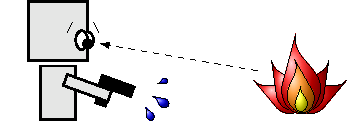
\includegraphics[scale=0.9]{robot_pompier}};
\node (bli) at (0,6.5) {};
}
\visible<2->{
\node (pomdp3) at (4.25,5.05) {\color{DodgerBlue!70}{$s \in \mathcal{S}$}: \color{black}{\textbf{system states}};};
\node (t1) at (2,5) {};
\node (r1) at (-2.3,5.5) {};
\node (r11) at (1,4.5) {};
\draw[->,>=latex,color=DodgerBlue!70,thick] (t1) to (r1);
\draw[->,>=latex,color=DodgerBlue!60,thick] (t1) to[bend right] (r11);
}
\visible<3->{
\node (pomdp4) at (3.85,4.45) {\color{MediumAquamarine}{$o \in \mathcal{O}$:} \color{black} \textbf{observations};};
\node (t2) at (2,4.4) {};
\node (r2) at (-2.3,5.05) {};
\draw[->,>=latex,color=MediumAquamarine,thick] (t2) to[bend left] (r2);
}
\visible<4->{
\node (pomdp5) at (4.4,3.85) {\color{MediumPurple}{$a \in \mathcal{A}$:} \color{black} \textbf{agent's actions};};
\node (t3) at (2,3.9) {};
\node (r3) at (-2,4.2) {};
\draw[->,>=latex,color=MediumPurple,thick] (t3) to[bend left] (r3);
}
\visible<8->{
\node (pomdp6) at (3.95,3.3) {\color{red}{$b$}: \color{black} \textbf{belief state}.};
}
\end{tikzpicture}
\vspace{-1cm}
\begin{tikzpicture}[scale=0.78,transform shape]
%%%%%%%%%%%%%%%%%%%%%%%%%%%%%%%%%%%%%%%%%%%%%%%%%%%%%%%%%%%%%%%%%%%%%%%%
%vis1: state
%%%%%%%%%%%%%%
%%%%%%%%%%%%%%
%\node (bli) at (0,0.5) {};
\visible<5->{
\tikzstyle{mvertex}=[circle,fill=black!60,minimum size=30pt,inner sep=0pt]
\node[mvertex] (state1t) at (3,0) {$s_t$};
\node[fill=black!30] (action) at (6.3,-1.7) {$a_t$};
\node[mvertex] (state2t) at (7.7,0) {$s_{t+1}$};
\tikzstyle{bvertex}=[circle,fill=red!60,minimum size=30pt,inner sep=0pt]
%1->2
\draw[->,>=latex] (state1t) -- (state2t);
\draw[->,>=latex] (action) -- (state2t);
\node (pisasp) at (6,-0.3) {$\textbf{p} \hspace{-0.05cm} \paren{ \hspace{-0.05cm} s_{t+1} \hspace{-0.05cm} \sachant \hspace{-0.05cm} s_{t}, \hspace{-0.05cm} a_t \hspace{-0.05cm} }$};
\node[fill=black!30] (hobserv2) at (10.2,-3.3) {$o_{t+1}$};
\draw[->,>=latex] (state2t) to (hobserv2);
\draw[->,>=latex] (action) to  (hobserv2);
\node (pisvshaoh2) at (8.4,-2) [rotate=330] {$\textbf{p} \paren{ o_{t+1} \sachant s_{t+1},a_{t} }$};
\tikzstyle{rvertex}=[fill=yellow!60,minimum size=10pt,inner sep=0pt]
\node[rvertex] (Rtbis) at (5.3,-4.3) {\textbf{reward}};
\node[rvertex] (Rt) at (6.9,-4) {$r(s_t,a_t)$};
\draw[->,decorate,decoration={snake,amplitude=.4mm,segment length=2mm,post length=1mm}] (state1t) -- (Rt); 
\draw[->,decorate,decoration={snake,amplitude=.4mm,segment length=2mm,post length=1mm}] (action) -- (Rt); 
}

%visFIN:
%%%%%%%%%%%%%%
%%%%%%%%%%%%%%
\visible<6->{
%s
\node (state0) at (0,0) {};
\node (state3) at (13,0) {};
\node (state0bis) at (0,-1.8) {};
\node (state3bis) at (13,-0.5) {};
\node (obs3) at (13,-2.3) {};
\draw[->,>=latex,dashed] (state0) -- (state1t);
\draw[->,>=latex,dashed] (state2t) -- (state3);
\node (pisasp2) at (1.1,-0.3) {$\textbf{p} \hspace{-0.05cm} \paren{ \hspace{-0.05cm} s_{t} \hspace{-0.05cm} \sachant \hspace{-0.05cm} s_{t-1}, \hspace{-0.05cm} a_{t-1} \hspace{-0.05cm} }$};
%a
\node[fill=black!30] (action0) at (1.6,-1.7) {$a_{t-1}$};
\draw[->,>=latex] (action0) -- (state1t);
\node[fill=black!30] (actiontp1) at (11.5,-1.7) {$a_{t+1}$};
\draw[->,>=latex,dashed] (actiontp1) -- (state3bis);
\draw[->,>=latex,dashed] (actiontp1) -- (obs3);
%o
\node (pisvshaoh1) at (3.9,-2.15) [rotate=330] {$\textbf{p} \paren{ o_{t} \sachant s_t,a_{t-1} }$};
\node[fill=black!30] (hobserv1) at (5.5,-3.3) {$o_{t}$};
\draw[->,>=latex] (state1t) to (hobserv1);
\draw[->,>=latex] (action0) to  (hobserv1);
%r
\node[rvertex] (Rt2) at (11.8,-4) {$r(s_{t+1},a_{t+1})$};
\draw[->,decorate,decoration={snake,amplitude=.4mm,segment length=2mm,post length=1mm}] (state2t) -- (Rt2); 
\draw[->,decorate,decoration={snake,amplitude=.4mm,segment length=2mm,post length=1mm}] (actiontp1) -- (Rt2); 

\node[rvertex] (Rt3) at (2,-4) {$r(s_{t-1},a_{t-1})$};
\draw[->,decorate,decoration={snake,amplitude=.4mm,segment length=2mm,post length=1mm}] (state0bis) -- (Rt3); 
\draw[->,decorate,decoration={snake,amplitude=.4mm,segment length=2mm,post length=1mm}] (action0) -- (Rt3);
}

\visible<7->{
	\coordinate (A) at (0,-1); 
	\coordinate (B) at (13,-1); 
	\coordinate (C) at (13,-3.7);
	\coordinate (D) at (0,-3.7); 
	\fill[red!20,opacity=0.5] (A) -- (B) -- (C) -- (D) -- cycle;
}

%visFINFIN belief
%%%%%%%%%%%%%
%%%%%%%%%%%%%
\visible<8->{
\node (bel0) at (1,1) {};
\node (bel3) at (13,1) {};
\node[bvertex] (bel2) at (10.5,1) {$b_{t+1}$};
\node[bvertex] (bel1) at (5.8,1) {$b_{t}$};
\node (pbb) at (8.25,1.3) [color=red,thick] {$\textbf{p} \paren{ b_{t+1} \sachant b_t,a_{t} }$};
\draw[->,>=latex,color=red,thick] (bel1) to (bel2);
\draw[->,>=latex,color=red,dashed,thick] (bel0) to (bel1);


\draw[->,>=latex,color=red,dashed,thick] (bel2) to (bel3);

%\node (procBel) at (12.7,0.1) [color=red] {croyance $b_{t+1}$ telle que};
%\node (procBelp) at (12.8,-0.4) [color=red] {$b_{t+1}(s_{t+1}) = \textbf{p} \paren{ s_{t+1} \sachant history }$.};
%\node (procBel2) at (12.8,-1.2) [color=red] {\textbf{règle de Bayes} $\rightarrow$ le calcul };
%\node (procBel3) at (12.8,-1.7) [color=red] { utilise $o_{t+1}$, $a_t$ et $b_t$ };

\draw[->,>=latex,color=red,thick] (hobserv2) to[bend left] (bel2);
\draw[->,>=latex,color=red,thick] (action) to (bel2);
\draw[->,>=latex,color=red,thick] (hobserv1) to[bend left] (bel1);
\draw[->,>=latex,color=red,thick] (action0) to (bel1);
}
\end{tikzpicture}
\end{frame}

\begin{frame}
\definecolor{bblue}{rgb}{0,0.4,0.75}
	\frametitle{\insertsection} 
	\framesubtitle{\footnotesize belief state, strategy, criterion.}
\center \textbf{POMDP:} $\langle \mathcal{S}, \mathcal{A}, \mathcal{O}, T, O, r, \gamma \rangle$,
\begin{itemize}
\item \textbf{transition} function $T(s,a,s') = \textbf{p} \paren{ s' \sachant s, a }$;
\item \textbf{observation} function $O(s',a,o') = \textbf{p} \paren{ o' \sachant s', a }$.
\end{itemize}
\vspace{1cm}
\visible<2->{
\[ { \textbf{belief state: }  \color{bblue} \displaystyle b_{t}(s) = \mathbb{P} \paren{ s_t = s \sachant a_0, o_1, \ldots, a_{t-1}, o_t  } } \]
}
\visible<3->{
\begin{exampleblock}{\textbf{probabilistic} belief update}
\begin{center}
$ b_{t+1}(s') %= u(b_t,a,o') 
\propto \textbf{p} \paren{ o' \sachant s',a} \cdot \sum_{s \in \mathcal{S}} \textbf{p} \paren{ s' \sachant s,a} \cdot b_t(s)  $
\end{center}
\end{exampleblock}
\vspace{-0.15cm}
\visible<4->{
\begin{block}{action choices: strategy $\delta(b_t) = a_t \in \mathcal{A}$}
\begin{center}
maximizing $ \displaystyle \mathbb{E}_{s_0 \sim b_0} \croch{ \sum_{t=0}^{+ \infty} \gamma^t \cdot r\Big(s_t,\delta(b_t)\Big) }$, $0<\gamma<1$. 
\end{center}
\end{block}
}
}

\end{frame}

\begin{frame}
\frametitle{Flaws of the POMDP model}
\framesubtitle{\footnotesize POMDPs in practice}
\begin{itemize}
\item optimal strategy computation $\geqslant$ \textbf{PSPACE};
\end{itemize}
\begin{itemize}
%\rightarrow raisonnement sur l'ensemble des probabilités $b \in \mathcal{B}_{\mathcal{S}}$
\item probabilities are \textbf{imprecisely known} in practice;
% \textit{ex:} $o \in \mathcal{O}$ sorties d'algorithmes de vision artificielle:\\
%fonction $O$ dépendante des datasets; 
\end{itemize}
%grande variabilité d'images $\rightarrow$ classifieur dur à extraire;\\
%$\# \mathcal{O}$ plus grand $\rightarrow$ POMDP plus complexe.
%\item définition de la fonction d'observation $O$?
\begin{itemize}
% ignorante?\\
%quantification si imprécision?
%\end{itemize}
%\begin{itemize}
\item agent's \textbf{ignorance} not taken into account.
\end{itemize}
%mission d'observation $+$ situation inconnue;\\
%paramètres ``situation très peu probable''.
\end{frame}

\begin{frame}
\definecolor{bblue}{rgb}{0,0.4,0.75}
\frametitle{Why model ignorance?}
\framesubtitle{\footnotesize knowledge is not always encouraged with POMDPs}
\begin{itemize}
\item initial belief deterministic $s_0=s_A$.
\end{itemize}
\vspace{0.1cm}
\begin{tikzpicture}

\tikzstyle{avertex}=[circle,fill=green!30,minimum size=20pt,inner sep=0pt]
\tikzstyle{vertex}=[circle,fill=black!30,minimum size=20pt,inner sep=0pt]

\visible<2->{
\node (L) at (-1,0) {};
\node (R) at (8.5,0) {};
\draw[thick,dashed,color=black!30] (L) to (R);
}

\node[vertex] (sA) at (0,0) {$s_A$};
\node[fill=bblue!30] (b0) at (-0.7,-0.8) {$b_0(s_A) = 1$};

\visible<2->{
\node[avertex] (a1) at (1,1.5) {$a'$};
\node[vertex] (sB) at (3,2) {$s_B$};
\node[fill=bblue!30] (b1A) at (5,2) {$b_1(s_B) = 0.5$};
\node[vertex] (sC) at (3,1) {$s_C$};
\node[fill=bblue!30] (b1B) at (5,1) {$b_1(s_C) = 0.5$};
\node[fill=yellow] (rA) at (8,2) {$r(s_B)=10$};
\node[fill=yellow] (rB) at (8,1) {$r(s_C)=0$};
\draw[->,>=latex,thick,color=red] (sA) to (sB);
\draw[->,>=latex,thick,color=red] (sA) to (sC);
}
\visible<3->{
\node[avertex] (a2) at (1,-1.5) {$\tilde{a}$}; 
\node[vertex] (sD) at (3,-1) {$s_D$};
\node[fill=bblue!30] (b1C) at (5,-1) {$b_1(s_D) = 1$};
\node[fill=yellow] (rC) at (8,-1) {$r(s_D)=5$};
\draw[->,>=latex,thick,color=blue] (sA) to (sD);
}
\end{tikzpicture}
\visible<4->{
\vspace{-0.5cm}
\begin{itemize}
\item $ \set{ s_B, s_C, s_D }$ $\xrightarrow{\mbox{\scriptsize deterministic}} s_E$, $r(s_E)=0$.
\end{itemize}
}
\visible<5->{
\begin{block}{}
 $ \displaystyle \mathbb{E}_{s_0 \sim b_0} \croch{ \sum_{t=0}^{+ \infty} \gamma^t \cdot r(s_t) \sachant a_0 = { \color{red} \tilde{a} } \mbox{ or } { \color{red} a' } } = r(s_0) + 5 \gamma$. \\
\textbf{ the safe action is not prefered.}
\end{block}
}
\end{frame}


\begin{frame}
\frametitle{Qualitative Possibility Theory}
\framesubtitle{\footnotesize an hybrid model with possibilistic belief states}
\begin{block}{Qualitative Possibility Theory}
\begin{itemize}
\item \textbf{simplification}/\textbf{imprecision} taken into account,\\
{\color{red} BUT frequentist information lost};
\item \textbf{ignorance} modeling;
\item possibilistic belief states already studied: $\pi$-POMDP (Sabbadin UAI98, Drougard UAI13, AAAI14).
\end{itemize}
\end{block}
\visible<2->{
\begin{itemize}
\item \textbf{POMDP with possibilistic belief states}\\ 
$\rightarrow$ heuristic for solving POMDPs; \\
$\rightarrow$ results in a standard MDP.\\
%\item traduction PSCACE $\rightarrow$ EXPTIME car $\# \Pi_S \sim \# \mathcal{L}^{\# \mathcal{S}}$.
\end{itemize}
}
\visible<3->{
\begin{alertblock}{}
\begin{itemize}
\item {\color{red} defined distributions $\pi$}:\\
%\begin{enumerate}
%\item 
$\mathbb{P} \rightarrow \pi$ transformations: 
pignistic, specific, $\ldots$
%\item %probabilités estimées avec garantie faible\\ 
%POMDP décrit plus fidèlement par $\pi$.
%\end{enumerate} 
\end{itemize}
\end{alertblock}
}
\end{frame}

\begin{frame}
\frametitle{Qualitative Possibility Theory}
\framesubtitle{\footnotesize presentation}
\vspace{0.15cm}
$1 = l_1 > l_2 > \ldots > l_{\# \mathcal{L}} = 0$ form the \textbf{finite scale} 
$\mathcal{L}$.
\begin{exampleblock}{}	
\flushleft events $e \subset \Omega$ (universe) \\ 
\centering
\textbf{sorted} using possibility \textbf{degrees} $\pi(e) \in \mathcal{L}$, \\
	$\neq$ \\
	\textbf{quantified} with \textbf{frequencies} $\textbf{p}(e) \in \croch{0,1}$ (probabilities).
	\end{exampleblock}
\visible<2->{
	\begin{block}{}
	$e_1 \neq e_2$, $2$ events $\subset \Omega$ 
	\begin{itemize}
	\item $ \pi(e_1) < \pi(e_2) $ $\Leftrightarrow$ \enquote{$e_1$ 
is less plausible than $e_2$}; \\
	\end{itemize}	
	\end{block}
}
	\visible<3->{ 
	\begin{alertblock}{}
	\centering
	{ \color{red} \hspace{1.2cm} Probability ($\mathbb{P}$) \hspace{0.3cm} / \hspace{0.1cm} Possibility ($\Pi$)}:
	\vspace{0.1cm}
	{\renewcommand{\arraystretch}{1.2} %donne la distance entre les lignes%
	{\setlength{\tabcolsep}{0.15cm} %donne la distance entre les collones%
	\resizebox{11cm}{!}{
	\begin{tabular}{!{\vrule width 2pt}c!{\vrule width 2pt}c!{\vrule width 1pt}c!{\vrule width 2pt}}
	\noalign{\hrule height 2pt} 
 	$e_1$ or $e_2$ &  $ \textbf{p}(e_1) + \textbf{p}(e_2 \cap 
\overline{e_1}) $  & $ \max \set{ \pi(e_1), \pi(e_2)}$ \\
	\noalign{\hrule height 2pt}  	
	$e_1$ and $e_2$ & $ \textbf{p}(e_1). \textbf{p} \paren{e_2 \sachant e_1 } $  & $\min \set{\pi(e_1), \pi(e_2 \sachant e_1)  }$ \\
	\noalign{\hrule height 2pt}  	
	\end{tabular}
	}
	}
	}
	\end{alertblock}	
	}
\end{frame}


\section{An hybrid POMDP}
\begin{frame}
\definecolor{bblue}{rgb}{0,0.4,0.75}
\frametitle{A possibilistic belief state}
\framesubtitle{\footnotesize belief space discretization }
\vspace{0.2cm}
$\Pi_{S} = \Big\{$ possibility distributions $\Big\}$: $\# \Pi_{S} < + \infty$\\ 
\vspace{0.1cm} 
$\rightarrow $ \textbf{belief space discretization}.
\vspace{-0.1cm}
\visible<2->{
\[ { \color{bblue}  b^{\pi}_{t} (s) = \pi \paren{ s_t = s \sachant a_0,o_1, \ldots, a_{t-1}, o_t } } \]
}
\vspace{-0.6cm}
\visible<3->{
\begin{exampleblock}{update -- \textbf{possibilistic} belief state}
\vspace{0.1cm}
$b^{\pi}_{t+1}(s')  %= u(b^{\pi}_{t},a,o')(s') 
=  \left \{ \begin{array}{ccc} 1 & \hspace{-1cm} \mbox{ if } \pi \paren{ o',s' \sachant b_t^{\pi}, a} = \pi \paren{ o' \sachant b_t^{\pi}, a} \\
\pi \paren{ o', s' \sachant b_t^{\pi}, a} & \mbox{ otherwise.}  
\end{array} \right.$ \\
\vspace{0.3cm}
${ \color{red} \mbox{ denoted by } }  { b^{\pi}_{t+1}(s') \color{red} \propto^{\pi} \pi \paren{o',s'\sachant b_t^{\pi}, a}} $
\end{exampleblock}
}
\visible<4>{
\begin{itemize}
\item $\displaystyle  \pi ( o', s' \vert b_t^{\pi}, a)  = \max_{s \in \mathcal{S}} \min \Big\{ \pi ( o' \vert s', a ), \pi ( s' \vert s, a ), b^{\pi}_t(s) \Big\}$;
\item $ \displaystyle \pi \paren{o' \sachant s', a} = \max_{s' \in \mathcal{S} } \pi \paren{ o',s' \sachant b^{\pi}_t, a  }$.
\end{itemize}
}
\vspace{-0.2cm}
\visible<5->{
\begin{block}{}
\begin{itemize}
\item the update \textbf{only depends on $o'$ and $a$}.
\end{itemize}
\end{block}
}
\end{frame}

\begin{frame}
\frametitle{Pignistic transformation and transitions}
\framesubtitle{\footnotesize Pignistic transformation}
numbering of the $n = \# \mathcal{S}$ system states:
$1 = b^{\pi}(s_1) \geqslant \ldots \geqslant b^{\pi}(s_{n}) \geqslant b^{\pi}(s_{n+1}) = 0$.
\begin{exampleblock}{\textbf{pignistic transformation} -- $P: \Pi_{\mathcal{S}} \rightarrow \mathbb{P}_{S} $}
\[ \overline{b^{\pi}}(s_i) = \sum_{j=i}^{\# \mathcal{S}} \frac{b^{\pi}(s_j) - b^{\pi}(s_{j+1})}{j}.\]
\end{exampleblock}
\begin{itemize}
\item probability distribution $\overline{b^{\pi}}$ $=$ \textbf{gravity center} \\ 
\hspace{1cm} of the represented probabilistic distributions;
%induites par la distribution de possibilité $b^{\pi}$ 
\item \textbf{Laplace principle}: ignorance $\rightarrow$ uniform probability.
\end{itemize}
%\begin{tikzpicture} 
%\draw [domain=-7:-1] plot(\x,0);
%\draw [domain=-2:2, scale=0.6] plot (\x-7.5,{exp(-\x*\x)});
%\draw [domain=-2:3, scale=0.6] plot (\x-7.5,{0.5*exp(-\x*(\x-2))});
%\node (poss) at (-3,0.5) {$\pi$};
%\node (pref) at (-5.5,0.5) {$\mu$};
%\node (S) at (-7.5,0) {$S$};
%\draw [domain=-2:2] plot(\x,0);
%\draw [domain=-1:0.35, scale=0.6, color=red] plot (\x-1,{0.5*exp(-\x*(\x-2))});
%\draw [domain=0.35:2, scale=0.6, color=red] plot (\x-1,{exp(-\x*\x)});
%\draw [domain=-2:0.35, scale=0.6, color=blue] plot (\x-1,{exp(-\x*\x)});
%\draw [domain=0.35:3, scale=0.6, color=blue] plot (\x-1,{0.5*exp(-\x*(\x-2))});
%\node [color=red] (inter) at (-0.5,-0.2) {$f_{\textbf{P} \cap \textbf{M}}$};
%\node [color=blue] (union) at (-1.5,0.7) {$f_{\textbf{P} \cup \textbf{M}}$};
%\end{tikzpicture}
\end{frame}

\begin{frame}
\frametitle{Pignistic transformation}
\framesubtitle{\footnotesize Examples of pignistic transformations (red) of possibility distributions (blue)}
\end{frame}

\begin{frame}
\frametitle{Pignistic transformation and transitions}
\framesubtitle{\footnotesize Transition function of epistemic states}
Approximation of the probabilities over the observations:
\begin{itemize}
\item $\textbf{p} \paren{ o' \sachant s,a } = \sum_{s' \in \mathcal{S}} O(s',a,o') \cdot T(s,a,s');$
\item { \color{red} $ \displaystyle \textbf{p}\paren{o'\sachant b^{\pi},a} := \sum_{s\in\mathcal{S}}\textbf{p}\paren{o' \sachant s,a}\cdot\overline{b^{\pi}}(s)$.}
\end{itemize}
\begin{block}{}
\[ \Rightarrow \textbf{p} \Big( (b^{\pi})' \Big\vert b^{\pi},a \Big) = \sum_{ \substack{ o' \mbox{ \footnotesize t.q. } \\ u(b^{\pi},a,o')=(b^{\pi})'} }\textbf{p}\paren{o'\sachant b^{\pi},a}.\]
\end{block}
\vspace{0.5cm}
notation: if $a \in \mathcal{A}$ selected, $o' \in \mathcal{O}$ received,\\ 
\[ b^{\pi}_{t+1} = u \paren{o',a,b^{\pi}_t} = \mbox{ update of } b^{\pi}_t. \]
\end{frame}



\begin{frame}
\frametitle{Choquet integral and rewards}
\framesubtitle{\footnotesize pessimistic evaluation of the rewards -- 
necessity measure}
imprecision of $b^{\pi}$ $=$ agent ignorance $+$ discretization: 
\textbf{pessimistic reward} about these imprecisions.
\visible<2->{
\vspace{-0.15cm}
\begin{alertblock}{Dual measure of $\Pi:2^{\mathcal{S}} \rightarrow \mathcal{L}$}
necessity $\mathcal{N}$ such that
$\forall A \subseteq \mathcal{S}$, $\mathcal{N}(A) = 1 - \Pi(\overline{A})$.
\end{alertblock}
}
\visible<3->{
\vspace{-0.1cm}
%$a \in \mathcal{A}$ fixé:
$r_1 \hspace{-0.1cm} > \hspace{-0.1cm} r_2 > \hspace{-0.1cm} \ldots \hspace{-0.1cm} > \hspace{-0.1cm} r_{k+1} \hspace{-0.05cm}= \hspace{-0.05cm}0$ represents elements of
$\big\{ \hspace{-0.02cm} r(s,a) \hspace{-0.02cm} \big\vert \hspace{-0.02cm} s \in \mathcal{S} \hspace{-0.02cm} \big\}$. %$k \leqslant \# \mathcal{S}$.\\
\vspace{-0.15cm}
\begin{block}{Choquet integral of $r$ with respect to $\mathcal{N}$}
\vspace{-0.6cm}
\begin{eqnarray}
Ch(r,\mathcal{N}) & = & \displaystyle \sum_{i=1}^{k} (r_i - r_{i+1}) \cdot \mathcal{N} \paren{ \set{r(s) \geqslant r_i} }\\
\vspace{-0.1cm}
\visible<4->{
\label{choquet2} & = & \displaystyle \sum_{i=1}^{\# \mathcal{L}-1} (l_i - l_{i+1}) \cdot \hspace{-0.1cm} \min_{ \substack{ s \in \mathcal{S} \mbox{ \scriptsize  s.t. } \\ b^{\pi}(s) \geqslant l_i } }  r(s).
} 
\end{eqnarray}
\end{block}
\vspace{-0.1cm}
\visible<4->{
notation $\mathcal{L} = \set{ l_1=1,l_2,l_3, \ldots, 0 }$.
}
}
\end{frame}
\begin{frame}
\frametitle{Choquet integral and rewards}
\framesubtitle{\footnotesize back to the example about ignorance}
%\begin{itemize}
%\item croyance initiale deterministe $s_0=s_A$;\\
%\item $ \set{ s_B, s_C, s_D }$ $\xrightarrow{\mbox{\scriptsize déterministe}}s_E$, $r(s_E)=0$.
%\end{itemize}
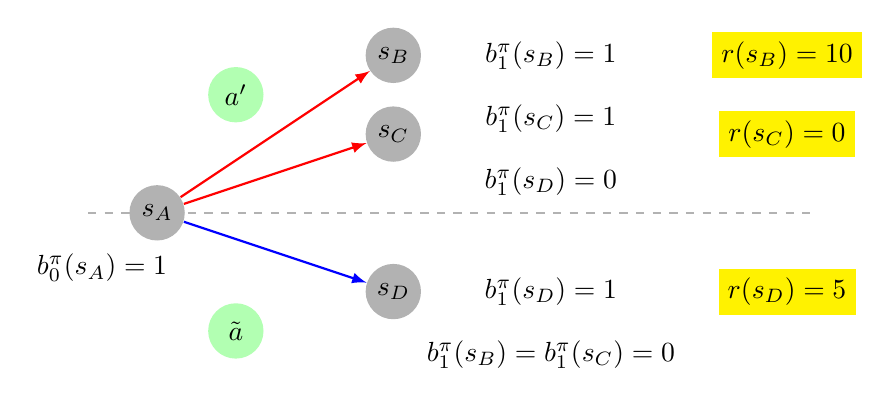
\begin{tikzpicture}
\node (L) at (-1,0) {};
\node (R) at (8.5,0) {};
\draw[thick,dashed,color=black!30] (L) to (R);
\tikzstyle{avertex}=[circle,fill=green!30,minimum size=20pt,inner sep=0pt]
\node[avertex] (a1) at (1,1.5) {$a'$};
\node[avertex] (a2) at (1,-1.5) {$\tilde{a}$}; 

\tikzstyle{vertex}=[circle,fill=black!30,minimum size=20pt,inner sep=0pt]
\node[vertex] (sA) at (0,0) {$s_A$};
\node (b0) at (-0.7,-0.7) {$b^{\pi}_0(s_A) = 1$};
\node[vertex] (sB) at (3,2) {$s_B$};
\node (b1A) at (5,2) {$b^{\pi}_1(s_B) = 1$};
\node[vertex] (sC) at (3,1) {$s_C$};
\node (b1B) at (5,1.2) {$b^{\pi}_1(s_C) = 1$};
\node (b1B) at (5,0.4) {$b^{\pi}_1(s_D) = 0$};
\node[vertex] (sD) at (3,-1) {$s_D$};
\node (b1C) at (5,-1) {$b^{\pi}_1(s_D) = 1$};
\node (b1C) at (5,-1.8) {$b^{\pi}_1(s_B) = b^{\pi}_1(s_C) = 0$};

\node[fill=yellow] (rA) at (8,2) {$r(s_B)=10$};
\node[fill=yellow] (rB) at (8,1) {$r(s_C)=0$};
\node[fill=yellow] (rC) at (8,-1) {$r(s_D)=5$};

\draw[->,>=latex,thick,color=red] (sA) to (sB);
\draw[->,>=latex,thick,color=red] (sA) to (sC);
\draw[->,>=latex,thick,color=blue] (sA) to (sD);
\end{tikzpicture}
\vspace{-0.8cm}
\visible<2->{
\begin{block}{}
% $\mathbb{E}_{s_0 \sim b_0} \croch{ r(s_1) \sachant a_0 = \tilde{a} } = \mathbb{E}_{b_0} \croch{ r(s_1) \sachant a' } = r(s_0) + \frac{\gamma}{2}$. \\
\begin{itemize}
\item $Ch \paren{ r, N_{b^{\pi}_1} \sachant a_0 = \tilde{a} } = r(s_D,\tilde{a}) = 5$, 
\item $Ch \paren{ r, N_{b^{\pi}_1} \sachant a_0 = a' } = \min_{s \in \mathcal{S}} r(s,a') = 0$. \\ 
\end{itemize}
the safe action is prefered! \textbf{dispersion reduced}
\end{block}
}
\visible<3->{	
if $\mathcal{N}_{b^{\pi}_1}$ replaced by $b_1$
$\Rightarrow$ $Ch(r,b_1) = \mathbb{E}_{s \sim b_1} \croch{r(s,a)}$.
% \sum_{s \in \mathcal{S}} r(s,a) \cdot b_1(s)$.
}
\end{frame}

\begin{frame}
\frametitle{resulting MDP}

\framesubtitle{\footnotesize translation summary}
\vspace{0.3cm}
input: a POMDP $\langle \mathcal{S},\mathcal{A},\mathcal{O},T,O,r, \gamma \rangle$; \\
output: the MDP $\langle \tilde{\mathcal{S}},\mathcal{A},\tilde{T},\tilde{r}, \gamma \rangle$:
\vspace{0.3cm}
\visible<2->{
\begin{itemize}
\item \textbf{state space} ${ \color{red} \tilde{\mathcal{S}} = \Pi_{\mathcal{S}} }$,\\ 
the set of the possibility distributions over $\mathcal{S}$;
\end{itemize}
}
\vspace{0.3cm}
\visible<3->{
\begin{itemize}
\item $\forall b^{\pi}, (b^{\pi})'$ possibilistic belief states $\in \Pi_{\mathcal{S}}$, $\forall a \in \mathcal{A}$,\\
\textbf{transitions} ${ \color{red} \tilde{T} \Big( b^{\pi}, a, (b^{\pi})' \Big) = \textbf{p} \Big( (b^{\pi})' \Big\vert b^{\pi},a \Big) }$;
\end{itemize}
}
\vspace{0.3cm}
\visible<4->{
\begin{itemize}
\item \textbf{reward} ${ \color{red}  \tilde{r}(a,b^{\pi}) = Ch \Big( r(a,.),\mathcal{N}_{b^{\pi}} \Big) }$,\\ 
$\mathcal{N}_{b^{\pi}}$ necessity measure computed from $b^{\pi}$.
\end{itemize}
}
\vspace{0.2cm}
\visible<5->{
\[ \mbox{ \textbf{criterion:} } \mathbb{E}_{ (b^{\pi}_t) \sim \tilde{T}} \croch{ \sum_{t=0}^{+ \infty} \gamma^t \cdot \tilde{r} \paren{ b^{\pi}_t,d_t } }.\]
}
\end{frame}

\begin{frame}
\frametitle{hybrid POMDP and $\pi$-POMDP}
\framesubtitle{\footnotesize differences with possibilistic models}
\begin{tabular}{|c||c|c|}
  \hline
  & hybrid POMDP  & $\pi$-POMDP \\
  \hline \hline
\hspace{-0.2cm} transitions \hspace{-0.2cm} & probabilities & qualitative possibility \\
  \hline
\hspace{-0.2cm} rewards \hspace{-0.2cm} & quantitative $\in \mathbb{R}$ & qualitative $\in \mathcal{L}$  \\
  \hline
\hspace{-0.2cm} situation \hspace{-0.2cm} & 
\begin{tabular}{c} -some imprecisions \\ -large POMDP \end{tabular} & few quantitative \\
  \hline
\hspace{-0.2cm} issues & $\pi$ definition & commensurability \\
  \hline
in practice & MDP & $\pi$-MDP\\
\hline
\end{tabular}
\\
\vspace{0.3cm}
\visible<2->{
\textbf{hybrid model:}
\begin{itemize}
\item only belief states are possibilistic:
\end{itemize}
$\rightarrow$ agent knowledge $=$ \textbf{possibility} distribution;
\begin{itemize}
\item probabilistic dynamics:
\end{itemize}
$\rightarrow$ \textbf{approximated} (prob.) transition between epistemic states. 
}
\end{frame}

\section{Benefiting from factorized structures}
\begin{frame}
\frametitle{factorized POMDP}
\framesubtitle{\footnotesize definition}
\begin{itemize}
\item $\mathcal{S}$ described by $\mathbb{S} = \set{ s_1, \ldots, s_m }$: $\mathcal{S} = s_1 \times \ldots \times s_m$.\\
Notation: $\mathbb{S}' = \set{s_1', \ldots, s_m'}$;
\end{itemize}
\visible<2->{
\begin{itemize}
\item \textbf{transition} function of $s_j'$,\\ 
$T_j^a(\mathbb{S}, s'_j) = \textbf{p} \paren{ s'_j \sachant \mathbb{S}, a}$,
$\forall j \in \set{1, \ldots, m}$ et $\forall a \in \mathcal{A}$;
\end{itemize}
}
\visible<3->{
\begin{itemize}
\item $\mathcal{O}$ described by $\mathbb{O}=\set{ o_1, \ldots, o_n }$: $\mathcal{O} = o_1 \times \ldots \times o_n$;
\end{itemize}
}
\visible<4->{
\begin{itemize}
\item \textbf{observation} function of $o_i'$,\\
$O_i^a(\mathbb{S}', o'_i) = \textbf{p} \paren{ o'_i \sachant \mathbb{S}', a}$,
$\forall i \in \set{1,\ldots,n}$ et $\forall a \in \mathcal{A}$.
\end{itemize}
}
\vspace{0.3cm}
\visible<5->{
\textbf{independences:} \\
\vspace{0.1cm}
$\rightarrow$ $ \forall s_i',s_j' \in \mathbb{S}'$, \hspace{0.55cm} $s_i' \perp\!\!\!\perp s_j' \ \vert \set{\mathbb{S}, a \in \mathcal{A} }$,\\
\vspace{0.3cm}
$\rightarrow$ $\forall o_i', o_j' \in \mathbb{O}'$, \hspace{0.3cm} $o_i' \perp\!\!\!\perp o_j' \ \vert \set{ \mathbb{S}', a \in \mathcal{A} }$.
}
\end{frame}

\begin{frame}
\frametitle{Notations}
\framesubtitle{\footnotesize some variables does not interact with each other}
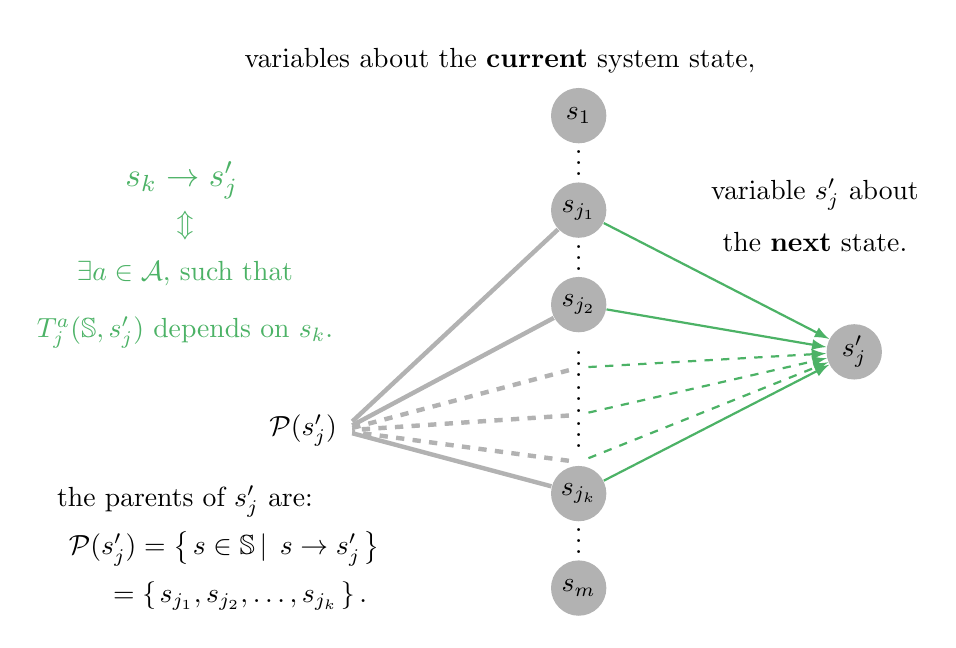
\begin{tikzpicture}
\node (legend0) at (-1,0.5) {};
\node (legend) at (-1,0.2) {variables about the \textbf{current} system state,};
\node (legend2) at (3,-1.5) {variable $s_j'$ about};
\node (legend3) at (3,-2.1) { the \textbf{next} state.};
\begin{scope}[scale=1.2,transform shape]
\visible<2->{
\node (A) at (-4.2,-1.1) { {\color[rgb]{0.3,0.7,0.4} $s_k \rightarrow s_j'$}};
}
\end{scope}

\definecolor{ggreen}{rgb}{0.3,0.7,0.4};
%	\node (legend2) at (-4,-0.6) {$s_k \thickrightarrow s_j'$};
\visible<2->{
\node (legend2) at (-5,-1.9) {{\color{ggreen} $\Updownarrow$}};
\node (legend2) at (-5,-2.5) {{\color{ggreen} $\exists a \in \mathcal{A}$, such that}};
\node (legend2) at (-5,-3.25) {{\color{ggreen} $T^a_j(\mathbb{S},s_j')$ depends on $s_k$.}};
}
%node
\tikzstyle{vertex}=[circle,fill=black!30,minimum size=20pt,inner sep=0pt]
\node[vertex] (s1) at (0,-0.5) {$s_1$};
\node (dots1) at (0,-1) {$\vdots$};
\node[vertex] (sk1) at (0,-1.7) {$s_{j_1}$};
\node (dots2) at (0,-2.2) {$\vdots$};
\node[vertex] (sk2) at (0,-2.9) {$s_{j_2}$};
\node (skF1) at (0,-3.7) {};
\node (skF2) at (0,-4.3) {};
\node (skF3) at (0,-4.9) {};
\node (dots3) at (0,-3.55) {$\vdots$};
\node (dots3) at (0,-4) {$\vdots$};
\node (dots3) at (0,-4.45) {$\vdots$};
\node[vertex] (sk3) at (0,-5.3) {$s_{j_k}$};
\node (dots4) at (0,-5.8) {$\vdots$};
\node[vertex] (sm) at (0,-6.5) {$s_m$};
\node[vertex] (spj) at (3.5,-3.5) {$s_j'$};
\visible<2->{
%draw
\draw[->,>=latex,thick,color=ggreen] (sk1) to (spj);
\draw[->,>=latex,thick,color=ggreen] (sk2) to (spj);
\draw[->,>=latex,thick,dashed,color=ggreen] (skF1) to (spj);
\draw[->,>=latex,thick,dashed,color=ggreen] (skF2) to (spj);
\draw[->,>=latex,thick,dashed,color=ggreen] (skF3) to (spj);
\draw[->,>=latex,thick,color=ggreen] (sk3) to (spj);
}
\visible<3->{
%legend
%\tikzstyle{point}=[circle,fill=black]
\node (nearP) at (-3,-4.5) {};
\draw[ultra thick,color=black!30] (sk1) to (nearP);
\draw[ultra thick,color=black!30] (sk2) to (nearP);
\draw[ultra thick,dashed,color=black!30] (skF1) to (nearP);
\draw[ultra thick,dashed,color=black!30] (skF2) to (nearP);
\draw[ultra thick,dashed,color=black!30] (skF3) to (nearP);
\draw[ultra thick,color=black!30] (sk3) to (nearP);
 
\node (parents) at (-3.5,-4.5) {$\mathcal{P}(s_j')$};
\node (parents2) at (-5,-5.4) {the parents of $s_j'$ are:};
\node (parents2) at (-4.5,-6) {$\mathcal{P}(s_j') = \set{ s \in \mathbb{S} \sachant s \rightarrow s_j'} $};
\node (parents3) at (-4.3,-6.6) {$ = \set{ s_{j_1}, s_{j_2}, \ldots,s_{j_k} }.$};
}
%\begin{scope}[scale=6,transform shape]
%\node (A) at (-0.1,-0.42) {$\{$};
%\end{scope}
\end{tikzpicture}
\end{frame}

\begin{frame}
\vspace{0.25cm}
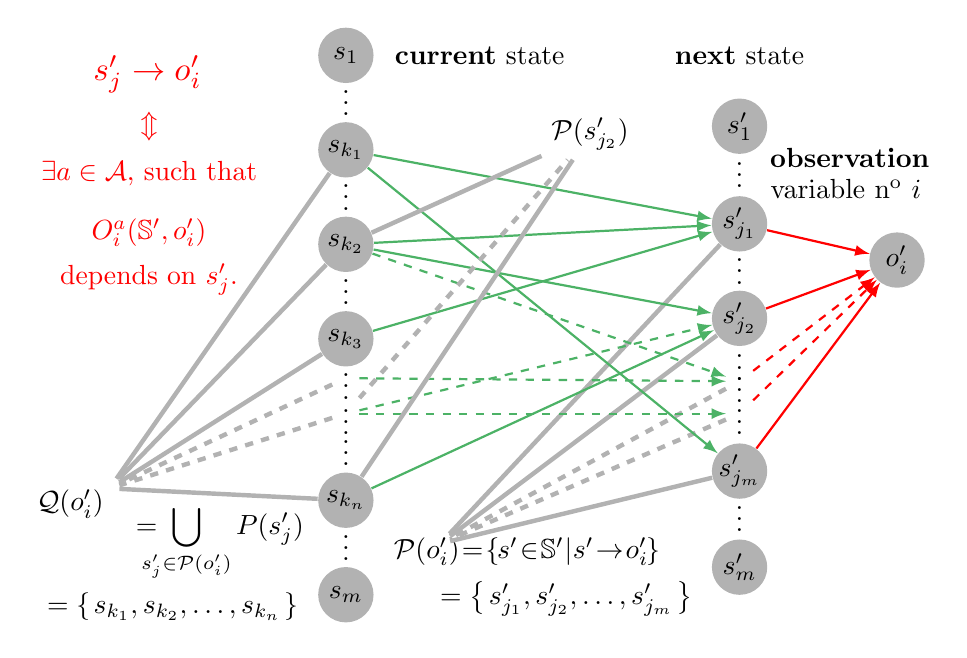
\begin{tikzpicture}
\definecolor{ggreen}{rgb}{0.3,0.7,0.4};
\frametitle{Notations}
\framesubtitle{\footnotesize concerning observation variables}
\visible<2->{
\begin{scope}[scale=1.2,transform shape]
\node (A) at (-2.1,-0.2) { {\color{red} $s_j' \rightarrow o_i'$}};
\end{scope}
\node (legend2) at (-2.5,-0.9) {{\color{red} $\Updownarrow$}};
\node (legend2) at (-2.5,-1.5) {{\color{red} $\exists a \in \mathcal{A}$, such that}};
\node (legend2) at (-2.5,-2.25) {{\color{red} $O^a_i(\mathbb{S}',o_i')$}};
\node (legend2) at (-2.5,-2.85) {{\color{red} depends on $s_j'$.}};
}
\tikzstyle{vertex}=[circle,fill=black!30,minimum size=20pt,inner sep=0pt]
\visible<4->{
\node (led) at (1.7,0) {\textbf{current} state};
\node[vertex] (s1) at (0,0) {$s_1$};
\node (dots1) at (0,-0.5) {$\vdots$};
\node[vertex] (sk1) at (0,-1.2) {$s_{k_1}$};
\node (dots2) at (0,-1.7) {$\vdots$};
\node[vertex] (sk2) at (0,-2.4) {$s_{k_2}$};
\node (dots3) at (0,-2.9) {$\vdots$};
\node[vertex] (sk3) at (0,-3.6) {$s_{k_3}$};
\node (dots4) at (0,-4.1) {$\vdots$};
\node (dots5) at (0,-4.55) {$\vdots$};
\node (dots6) at (0,-4.95) {$\vdots$};
\node[vertex] (sk4) at (0,-5.65) {$s_{k_n}$};
\node (dots7) at (0,-6.15) {$\vdots$};
\node[vertex] (sm) at (0,-6.85) {$s_m$};
}
\node (led) at (5,0) {\textbf{next} state};
\node[vertex] (sp1) at (5,-0.9) {$s_1'$};
\node (dotsp1) at (5,-1.42) {$\vdots$};
\node[vertex] (spj1) at (5,-2.14) {$s'_{j_1}$};
\node (dotsp2) at (5,-2.64) {$\vdots$};
\node[vertex] (spj2) at (5,-3.34) {$s'_{j_2}$};
\node (dotsp3) at (5,-3.86) {$\vdots$};
\node (dotsp5) at (5,-4.14) {$\vdots$};
\node (dotsp6) at (5,-4.55) {$\vdots$};
\node[vertex] (spj3) at (5,-5.28) {$s'_{j_m}$};
\node (dotsp4) at (5,-5.78) {$\vdots$};
\node[vertex] (smp) at (5,-6.5) {$s'_m$};

\visible<3>{
\node (poi) at (2.3,-6.3) {$\mathcal{P}(o_i') \hspace{-0.07cm} = \hspace{-0.07cm} \set{ \hspace{-0.07cm} s' \hspace{-0.07cm} \in \hspace{-0.07cm} \mathbb{S}' \hspace{-0.05cm} \sachant \hspace{-0.15cm} s' \hspace{-0.07cm} \rightarrow \hspace{-0.07cm} o_i' \hspace{-0.07cm}} $};
\node (h2) at (2.8,-6.9) { $= \set{ s'_{j_1}, s'_{j_2}, \ldots, s'_{j_m} }$};

\visible<3>{
\node (nearP) at (1.2,-6.2) {};
\draw[ultra thick,color=black!30] (spj1) to (nearP);
\draw[ultra thick,color=black!30] (spj2) to (nearP);
\draw[ultra thick,color=black!30] (spj3) to (nearP);
\draw[ultra thick,dashed,color=black!30] (dotsp6) to (nearP);
\draw[ultra thick,dashed,color=black!30] (dotsp5) to (nearP);
}
}

\visible<5->{
\draw[->,>=latex,thick,color=ggreen] (sk1) to (spj1);
\draw[->,>=latex,thick,color=ggreen] (sk2) to (spj1);
\draw[->,>=latex,thick,color=ggreen] (sk3) to (spj1);
\draw[->,>=latex,thick,color=ggreen] (sk2) to (spj2);
\draw[->,>=latex,thick,color=ggreen] (sk4) to (spj2);
\draw[->,>=latex,thick,color=ggreen] (sk1) to (spj3);
\draw[->,>=latex,thick,dashed,color=ggreen] (dots4) to (dotsp5);
\draw[->,>=latex,thick,dashed,color=ggreen] (sk2) to (dotsp5);
\draw[->,>=latex,thick,dashed,color=ggreen] (dots5) to (dotsp6);
\draw[->,>=latex,thick,dashed,color=ggreen] (dots5) to (spj2);
}
\visible<-2>{
\node (o) at (6.4,-1.3) {\textbf{observation}};
\node (o) at (6.35,-1.7) {variable n\textsuperscript{o} $i$};
}
\node[vertex] (opi) at (7,-2.6) {$o'_{i}$};
\visible<2->{
\draw[->,>=latex,thick,color=red] (spj1) to (opi);
\draw[->,>=latex,thick,color=red] (spj2) to (opi);
\draw[->,>=latex,thick,color=red] (spj3) to (opi);
\draw[->,>=latex,thick,dashed,color=red] (dotsp5) to (opi);
\draw[->,>=latex,thick,dashed,color=red] (dotsp6) to (opi);
}
\visible<6>{
\node (nearPS) at (3.1,-1) {$\mathcal{P}(s_{j_2}')$};
\draw[ultra thick,color=black!30] (sk2) to (nearPS);
\draw[ultra thick,color=black!30] (sk4) to (nearPS);
\draw[ultra thick,dashed,color=black!30] (dots5) to (nearPS);
}

\visible<7->{
\node (parents) at (-3.5,-5.7) {$\mathcal{Q}(o_i')$}; 
\node (parents) at (-1.6,-6.2) {$ =\hspace{-0.3cm} \displaystyle \bigcup_{s_j' \in \mathcal{P}(o_i')} P(s_j')$}; 
\node (parents) at (-2.2,-7) {$ = \set{ s_{k_1},s_{k_2},\ldots,s_{k_n} }$};

\node (nearQ) at (-3,-5.5) {};
\draw[ultra thick,color=black!30] (sk1) to (nearQ);
\draw[ultra thick,color=black!30] (sk2) to (nearQ);
\draw[ultra thick,color=black!30] (sk3) to (nearQ);
\draw[ultra thick,dashed,color=black!30] (dots4) to (nearQ);
\draw[ultra thick,dashed,color=black!30] (dots5) to (nearQ);
\draw[ultra thick,color=black!30] (sk4) to (nearQ);
}
\end{tikzpicture}
\end{frame}

\begin{frame}
\frametitle{Rewritings of parameters}
\framesubtitle{\footnotesize \textbf{PROBABILISTIC} parameters}
\begin{itemize}
\item $T^a_j \paren{ \mathbb{S},s_j' } = T^a_j \paren{\mathcal{P}(s_j'),s_j'}$;
\item $O^a_i \paren{ \mathbb{S}',o_i' } = O^a_i \paren{\mathcal{P}(o_i'),o_i'}$.
\end{itemize}
\visible<2->{
\begin{block}{consequences on the joint distribution}
\vspace{-0.3cm}
\begin{align*}
\textbf{p} \paren{ o_i', \mathcal{P}(o_i') \sachant \mathbb{S}, a} & = O^a_i \paren{ \mathcal{P}(o_i'), o_i'} \cdot \displaystyle \prod_{s_j'\in\mathcal{P}(o_i')} T^a_i \paren{\mathcal{P}(s_j'),s_j'} \\
& = \textbf{p} \paren{ o_i', \mathcal{P}(o_i') \sachant \mathcal{Q}(o_i'), a}.
\end{align*}
\end{block}
}
\visible<3->{
\vspace{-0.2cm}
\begin{alertblock}{observation probabilities}
epistemic state % sur $\mathbb{S}$: $b^{\pi} \in \Pi_{S}$.
\vspace{-0.7cm}
\begin{equation*}
 b^{\pi}(\mathbb{S}) \xrightarrow{ \mbox{\footnotesize \textbf{marginalization}} }  b^{\pi}(\mathcal{Q}(o_i')) \xrightarrow{ \begin{array}{cc} \mbox{\footnotesize \textbf{pignistic}}
\vspace{-0.2cm}
\\
 \mbox{\footnotesize \textbf{transformation}} \end{array} } \overline{b^{\pi}}(\mathcal{Q}(o_i')) 
\end{equation*} 
\vspace{-0.5cm}
\[ { \color{red} \textbf{p} \paren{ o_i' \sachant b^{\pi}, a } } = \sum_{2^{\mathcal{P}(o_i')},2^{\mathcal{Q}(o_i')}} \textbf{p} \paren{ o_i', \mathcal{P}(o_i') \sachant \mathcal{Q}(o_i'), a} \cdot \overline{b^{\pi}}(\mathcal{Q}(o_i')) \]
\end{alertblock}
}
\end{frame}
\begin{frame}
\frametitle{Parameters rewritings}
\framesubtitle{\footnotesize \textbf{POSSIBILISTIC} parameters}
\begin{itemize}
\item $\pi \paren{ s_j' \sachant \mathbb{S}, a } = \pi \paren{s_j' \sachant \mathcal{P}(s_j'), a}$;
\item $\pi \paren{ o_i' \sachant \mathbb{S}', a } = \pi \paren{o_i' \sachant \mathcal{P}(o_i'), a}$.
\end{itemize}
\visible<2->{
\begin{alertblock}{marginal possibilistic belief states}
$\forall o_i' \in \mathbb{O}$,\\
$ \displaystyle b^{\pi}_{t+1} \Big( \hspace{-0.05cm} \mathcal{P}(o_i') \hspace{-0.05cm} \Big) \propto^{\pi}  \pi  \Big( o_i', \mathcal{P}(o_i') \Big\vert a_0,o_1, \ldots, a_{t-1}, o_{t} \Big)$ \\
\visible<3->{
\hspace{2.93cm} $\displaystyle = \max_{2^{\mathcal{Q}(o_i')}} \hspace{-0.05cm} \min \hspace{-0.07cm} \Bigg\{ \hspace{-0.07cm} \pi \hspace{-0.05cm} \Big( \hspace{-0.05cm} o_i', \hspace{-0.05cm} \mathcal{P}(o_i') \hspace{-0.02cm} \Big\vert \hspace{-0.02cm} \mathcal{Q}(o_i'), \hspace{-0.05cm} a \hspace{-0.05cm} \Big)\hspace{-0.05cm}, \hspace{-0.05cm} b^{\pi}_t \hspace{-0.05cm} \Big( \hspace{-0.05cm} \mathcal{Q}(o_i') \hspace{-0.05cm} \Big) \hspace{-0.1cm} \Bigg\}$\\
}
\visible<4->{
\hspace{5cm} denoted by { \color{red} $\pi \Big( o_i', \mathcal{P}(o_i') \Big\vert b^{\pi}_t, a \Big)$}.
}
\end{alertblock}
}
\end{frame}


\begin{frame}
\frametitle{Variable classification}
\framesubtitle{\footnotesize $3$ classes of state variables}%: extension des MOMDPs (Araya-L\'opez, Ong)}
\vspace{0.1cm}
\begin{tikzpicture}
\definecolor{violet}{rgb}{0.7,0.1,0.5};
\definecolor{orangee}{rgb}{1,0.7,0.1};
\definecolor{gggreen}{rgb}{0,0.7,0.7};
% separations
\node (T1) at (-1.5,8.4) {};
\node (B1) at (9,8.4) {};
\draw[thick,dashed,color=black!30] (B1) to (T1);
\node (T2) at (-1.5,5.1) {};
\node (B2) at (9,5.1) {};
\draw[thick,color=black!30] (B2) to (T2);

% variables
\tikzstyle{vertex}=[circle,fill=black!30,minimum size=20pt,inner sep=0pt]
\node (V) at (1,10) { \underline{variable:} \color{violet} visible $s_v \in \mathbb{S}_v$ };
\node[vertex] (vv) at (6.5,9.7) {$s_v'$};
\node (IHV) at (1.3,8) { {\color{gggreen} inferred hidden $ s_h \in \mathbb{S}_h$} };
\node[vertex] (ihv) at (6.5, 7.15) {$s_h'$};
\node (FHV) at (2,4.75) { {\color{orangee} fully hidden $s_f \in \mathbb{S}_f$}};
\node[vertex] (fhv) at (6.5,4) {$s_f'$};

\visible<2->{
% visible
\node[vertex] (ov) at (8.5,9.7) {$o_v'$};
\draw[->,>=latex,thick] (vv) to (ov);
\node at (7.5,10) {$s_v'= o_v'$};
}
\visible<3->{
\node (leg1) at (3.5,8.9) {  \color{violet} $\textbf{p} \paren{ s_v' \sachant b_t^{\pi},a } = \sum_{2^{\mathcal{P}(s_v')}} T^a \hspace{-0.04cm} \paren{ \mathcal{P}(s_v'), s_v'} \cdot \overline{b^{\pi}_t} \Big(\mathcal{P}(s_v') \Big).$ };
}
\visible<4->{
\node (leg1) at (2,9.5) { $\Leftrightarrow$ deterministic belief variable. };
}

\visible<5->{
% inférée
\tikzstyle{hvertex}=[circle,fill=black!10,minimum size=20pt,inner sep=0pt]
\node[vertex] (oh) at (8.5,7.15) {$o_i'$};
\draw[->,>=latex,thick] (ihv) to (oh);
\node[hvertex] (sh1) at (6.5,8) {$s_h^{a}$};
\node[hvertex] (sh2) at (6.8,6.2) {$s_h^{b}$};
\node[hvertex] (sh3) at (7.5,5.5) {$s_h^{c}$};
\draw[->,>=latex,thick,dashed] (sh1) to (oh);
\draw[->,>=latex,thick,dashed] (sh2) to (oh);
\draw[->,>=latex,thick,dashed] (sh3) to (oh);
}

\visible<6->{
\node (leg2) at (2,7.3) {$ {\color{gggreen} b^{\pi}_{t+1}(\mathcal{P}(o_i')) }= b^{\pi}_{t+1}(s_h,s_h^a,s_h^b,s_h^c)$};
}
\visible<7->{

\node (leg2) at (3.2,6.4) {$  {\color{gggreen} \propto^{\pi} \pi \Big( o_i', \mathcal{P}(o_i') \Big\vert b^{\pi}_t, a \Big)}.$}; 
%\node (leg2) at (2.5,6.3) { $ \displaystyle \propto^{\pi} \hspace{-0.1cm} \max_{2^{\mathcal{Q}(o_i')}} \hspace{-0.1cm} \Bigg\{ \hspace{-0.1cm} \pi \hspace{-0.05cm} \Big( \hspace{-0.05cm}  o_i', \hspace{-0.05cm}  \mathcal{P}(o_i') \hspace{-0.02cm}  \Big\vert \hspace{-0.02cm}  \mathcal{Q}(o_i'), \hspace{-0.05cm}  a \hspace{-0.05cm}  \Big), \hspace{-0.1cm}  b^{\pi}_t \hspace{-0.1cm}  \Big( \hspace{-0.1cm}  \mathcal{Q}(o_i') \hspace{-0.1cm} \Big) \hspace{-0.1cm}  \Bigg\}$.}; 
}
\visible<8->{
\node (leg2) at (2.5,5.5) { { \color{red} {\fontencoding{U}\fontfamily{futs}\selectfont\char 66\relax}} $\mathcal{P}(o_i')$ may contain visible variables.};
}

\visible<9->{
% inférée
\tikzstyle{hvertex}=[circle,fill=black!10,minimum size=20pt,inner sep=0pt]
\node[vertex] (oh) at (8.5,4) {$o_i'$};
\draw[->,>=latex,thick] (fhv) to (oh);
\node (cross) at (7.5,4) {
\includegraphics[scale=0.033]{crossCheck}};
}
\visible<10->{
% inférée
\node (leg3) at (3.3,3.05) { { \color{orangee} $b^{\pi}_{t+1}(s_f') = \displaystyle \max_{2^{\mathcal{P}(s_f')}} \min \bigg\{ \pi \big( s_f'  \big\vert  \mathcal{P}(s_f'), \hspace{-0.1cm} a \big) , b^{\pi}_{t} \big(\mathcal{P}(s_f') \big) \bigg\} $}.};
}
\visible<11->{
\node (leg3) at (2,4.25) {$\rightarrow$ observations don't };
\node (leg3) at (2,3.75) { inform belief state on $s_f'$.};
}
\end{tikzpicture}
\end{frame}



\nico{
%%%%%%%%%%%%%%%%%%%%%%%%%%%%% classification des variables version verticale
\begin{frame}
%\changepage{textheight}{textwidth}{evensidemargin}{oddsidemargin}{columnsep}{topmargin}{headheight}{headsep}{footskip}
%\changepage{}{}{0cm}{0cm}{}{}{}{}{}
\frametitle{Classification des variables}
\framesubtitle{\footnotesize $3$ catégories de variables d'état}%: extension des MOMDPs (Araya-L\'opez, Ong)}
\begin{tikzpicture}
\definecolor{ggreen}{rgb}{0.3,0.7,0.4};
% separations
\node (T1) at (2.1,10.5) {};
\node (B1) at (2.1,3) {};
\draw[thick,dashed,color=black!30] (B1) to (T1);
\node (T2) at (5.9,10.5) {};
\node (B2) at (5.9,3) {};
\draw[thick,color=black!30] (B2) to (T2);

% variables
\tikzstyle{vertex}=[circle,fill=black!30,minimum size=20pt,inner sep=0pt]
\node (V) at (0.1,10.15) {\underline{variable:} {\color{red} visible $\in \mathbb{S}_v$}};
\node[vertex] (vv) at (0.3,9.4) {$s_v'$};
\node (IHV) at (3.9,10.15) { {\color{red} cachée inférée $\in \mathbb{S}_h$}};
\node[vertex] (ihv) at (3.7, 9.4) {$s_h'$};
\node (FHV) at (8,10.15) { {\color{red} complètement cachée}};
\node (FHV2) at (9.2,9.7) {{\color{red}$\in \mathbb{S}_f$}};
\node[vertex] (fhv) at (8,9.4) {$s_f'$};

\visible<2->{
% visible
\node[vertex] (ov) at (0.3,8) {$o_v'$};
\draw[->,>=latex,thick] (vv) to (ov);
\node at (-0.5,8.7) {$s_v'=o_v'$};
}
\visible<3->{
\node (leg1) at (-0.3,7) {$\textbf{p} \paren{ s_v' \sachant b_t,a }$};
\node (leg1) at (0,6) {$= \hspace{-0.3cm} \displaystyle \sum_{2^{\mathcal{P}(s_v')}} \hspace{-0.1cm} T^a \hspace{-0.04cm} \paren{ \hspace{-0.04cm} \mathcal{P}(s_v') \hspace{-0.04cm} , \hspace{-0.06cm} s_v' \hspace{-0.1cm} } \hspace{-0.1cm}$};
\node (leg1) at (0.9,5.6) {$\cdot b_t(\mathcal{P}(s_v')).$};
}
\visible<4->{
\node (leg1) at (0.1,4.8) {$s_v'$ observable};
\node (leg1) at (0.15,4.3) {{\color{ggreen} $\rightarrow$ considérée comme}};
\node (leg1) at (0.15,3.7) {{\color{ggreen}  une variable de}};
\node (leg1) at (0.2,3.1) {{\color{ggreen} croyance déterministe.}};
}


\visible<5->{
% inférée
\tikzstyle{hvertex}=[circle,fill=black!10,minimum size=20pt,inner sep=0pt]
\node[vertex] (oh) at (3.7,8) {$o_i'$};
\draw[->,>=latex,thick] (ihv) to (oh);
\node[hvertex] (sh1) at (2.8,9.4) {$s_h^{a}$};
\node[hvertex] (sh2) at (4.5,9.4) {$s_h^{b}$};
\node[hvertex] (sh3) at (5.3,9.4) {$s_h^{c}$};
\draw[->,>=latex,thick,dashed] (sh1) to (oh);
\draw[->,>=latex,thick,dashed] (sh2) to (oh);
\draw[->,>=latex,thick,dashed] (sh3) to (oh);
}

\visible<6->{
\node (leg2) at (3.2,7) {$ b^{\pi}_{t+1}(\mathcal{P}(o_i'))$};
\node (leg2) at (4.1,6.4) {$= b^{\pi}_{t+1}(s_h,s_h^a,s_h^b,s_h^c)$};
}
\visible<7->{
\node (leg2) at (3.8,5.8) { \footnotesize utilisant $b^{\pi}_t(\mathcal{Q}(o_i'))$ et };
\node (leg2) at (4.1,5.3) { \footnotesize $\pi \paren{ o_i', \mathcal{P}(o_i') \sachant \mathcal{Q}(o_i'), a }$.}; 
}
\visible<8->{
\node (leg2) at (3.5,4.3) { { \color{red} {\fontencoding{U}\fontfamily{futs}\selectfont\char 66\relax}} {\color{ggreen} $\mathcal{P}(o_i')$ peut}};
\node (leg2) at (3.7,3.7) {{\color{ggreen} contenir des}};
\node (leg2) at (4,3.1) {{\color{ggreen} variables visibles.}};
}

\visible<9->{
% inférée
\tikzstyle{hvertex}=[circle,fill=black!10,minimum size=20pt,inner sep=0pt]
\node[vertex] (oh) at (8,8) {$o_i'$};
\draw[->,>=latex,thick] (fhv) to (oh);
\node (cross) at (8,8.75) {
\includegraphics[scale=0.033]{crossCheck}};
}
\visible<10->{
% inférée
\node (leg3) at (7.5,7) {$b_{t+1}(s_f') = \displaystyle \max_{2^{\mathcal{P}(s_f')}} $};
\node (leg3) at (7.7,6.2) {$ \displaystyle \min \hspace{-0.1cm} \Big\{ \pi \hspace{-0.04cm} \paren{ s_f' \hspace{-0.04cm} \sachant \hspace{-0.1cm} \mathcal{P}(s_f') \hspace{-0.04cm} , \hspace{-0.1cm} a}$};
\node (leg3) at (8.8,5.6) {$, b^{\pi}_{t} (\mathcal{P}(s_f')) \Big\}.$};
}
\visible<11->{
\node (leg3) at (7.8,4.3) {{\color{ggreen} $\rightarrow$ les observations}};
\node (leg3) at (7.8,3.7) {{\color{ggreen} n'influencent pas}};
\node (leg3) at (8,3.1) {{\color{ggreen} la croyance sur $s_f'$.}};
}
\end{tikzpicture}
\end{frame}

}

\begin{frame}
\frametitle{Possibilistic belief variables}
\framesubtitle{\footnotesize global belief state}
\definecolor{violet}{rgb}{0.7,0.1,0.5}
\definecolor{orangee}{rgb}{1,0.7,0.1}
\definecolor{gggreen}{rgb}{0,0.7,0.7}
\definecolor{bblue}{rgb}{0,0.4,0.75}
$\mathbb{O}_h = \mathbb{O} \setminus \mathbb{S}_v$.
\begin{block}{bound over the global belief state}
$b^{\pi}_{t+1}(\mathbb{S}') = \pi \paren{ \mathbb{S}' \sachant a_0,o_1, \ldots, a_{t},o_{t+1} } $
\end{block}
$ \leqslant \beta_{t+1}(\mathbb{S}')$\\
$\hspace{0.8cm} \displaystyle = \min \hspace{-0.1cm} \Bigg\{ \hspace{-0.1cm} 
{\color{violet} \min_{s_j' \in \mathbb{S}_v} \hspace{-0.1cm} \bigg[ \mathds{1}_{ \set{s_j'=o_j'}} \bigg]} \hspace{-0.1cm}, 
{\color{orangee} \min_{s_j' \in \mathbb{S}_f} \hspace{-0.1cm} \bigg[ b^{\pi}_{t+1}(s_j') \bigg]} \hspace{-0.1cm} , \hspace{-0.1cm} 
{\color{gggreen} \min_{o_i' \in \mathbb{O}_h} \hspace{-0.1cm} \bigg[ b_{t+1}^{\pi} \Big( \hspace{-0.1cm} \mathcal{P}(o_i') 
\hspace{-0.1cm} \Big) \bigg]} \hspace{-0.1cm}  \Bigg\} \hspace{-0.3cm}$\\
\visible<2->{
\vspace{1cm}
\begin{itemize}
\item $\beta_t = $ \textbf{less informative} version of the belief state: 
{\color{red} $b_t^{\pi} \leqslant \beta_t$};
\item computed using \textbf{marginal belief states} $\leftrightarrow$ { \color{red} factorization}.
\end{itemize}
}
%en possibiliste, pas besoin d'enlever les $\mathcal{P}(o_i')$ grâce au min!\\
%The possibilistic normalization, $\forall w \in 2^{\mathcal{P}(o_i')}$,
%$b'(w) = \left \{ \begin{array}{ccc} 1 \mbox{ if } w \in \operatorname*{argmax}_{v \in 2^{\mathcal{P}(o_i')}} \tilde{b}'(v); \\
% \tilde{b}'(w) \mbox{ otherwise} . \end{array} \right.$ 
\end{frame}

\begin{frame}
\definecolor{violet}{rgb}{0.7,0.1,0.5}
\definecolor{orangee}{rgb}{1,0.7,0.1}
\definecolor{gggreen}{rgb}{0,0.7,0.7}
\frametitle{Variables de croyance}
\framesubtitle{\footnotesize different according to the class of the variable}
\definecolor{bblue}{rgb}{0,0.4,0.75}
$\lambda=\# \mathcal{L}$
\visible<2->{
\begin{alertblock}{}
\begin{itemize}
\item {\color{violet} $\forall s'_{v} \in \mathbb{S}_v$, $1$} variable {\color{violet} $\beta'_{v}$} is enough.
\vspace{0.7cm}
\visible<3->{
\item $p_i = \# \mathcal{P}(o_i')$. \\ 
\vspace{0.4cm}
{ \color{gggreen} $ \forall o_i \in \mathbb{O} \setminus \mathbb{S}_v$,}
$\lambda^{2^{p_i}} - (\lambda-1)^{2^{p_i}}$ belief states,\\ 
\vspace{0.3cm}
$\Rightarrow { \color{gggreen} \lceil \log_2(\lambda^{2^{p_i}} - (\lambda-1)^{2^{p_i}}) \rceil}$ boolean variables {\color{gggreen} $\beta_h'$ }.
}
%$\tilde{b}'(\mathcal{P}(o_i')) = \max_{v \in 2^{\mathcal{Q}(o_i')}} \min \set{ \pi \paren{ o_i', \mathcal{P}(o_i') \sachant v,a}, b(v) }$;
\vspace{0.7cm}
\visible<4->{
\item  { \color{orangee} $\forall s'_{f} \in \mathbb{S}_f$,} $\lambda^2 - (\lambda-1)^2 = 2\lambda-1$ belief states,\\ 
\vspace{0.2cm}
$\Rightarrow { \color{orangee} \lceil \log_2(2\lambda-1) \rceil }$ boolean variables {\color{orangee} $\beta_f'$}.
}
\end{itemize}
%where $\pi \paren{ o_i', \mathcal{P}(o'_i) \sachant \mathcal{Q}(o'_i), a }$ 
%$ = \min \set{ \pi \paren{ o_i' \sachant \mathcal{P}(o'_i), a}, \min_{s'_j \in \mathcal{P}(o'_i)} \pi \paren{ s'_j \sachant \mathcal{P}(s'_j), a  } }$.
\end{alertblock}
}
\end{frame}

\begin{frame}
\definecolor{violet}{rgb}{0.7,0.1,0.5}
\definecolor{orangee}{rgb}{1,0.7,0.1}
\definecolor{gggreen}{rgb}{0,0.7,0.7}
\frametitle{resulting MDP in practice}
\framesubtitle{\footnotesize trick: ``flipflop'' variable}

\begin{block}{}
boolean variable ``\textit{flipflop}'' $f$ 
changes state at each time step\\ 
$\rightarrow$ defines $2$ phases:
\begin{enumerate}
\item \textit{observation generation}, 
\item \textit{belief update} (deterministic knowing the observation). 
\end{enumerate}
\end{block}
MDP variables:\\ 
\vspace{0.3cm}
$\tilde{\mathbb{S}} =$ \\
 \textbf{beliefs}: \hspace{-0.2cm} $\beta = { \color{violet} \beta^1_v \hspace{-0.05cm} \times \hspace{-0.05cm} \ldots \hspace{-0.05cm} \times \hspace{-0.05cm} \beta^{m_v}_v } \times  { \color{gggreen} \beta^1_h \hspace{-0.05cm} \times \hspace{-0.05cm} \ldots \hspace{-0.05cm} \times \hspace{-0.05cm} \beta^{m_h}_h } \hspace{-0.07cm} \times { \color{orangee} \beta^1_f \hspace{-0.05cm} \times \hspace{-0.05cm} \ldots \hspace{-0.05cm} \times \hspace{-0.05cm} \beta^{m_f}_f } $ \\
\vspace{0.15cm}
\hspace{2cm} $\times$ \\
$ \begin{array}{c} \mbox{\textbf{visible}} \\ \mbox{\textbf{variables}} \end{array} $: $v = f \times { \color{violet} s^1_v \times \ldots \times s^{m_v}_v } \times o_1 \times \ldots \times o_{k} $.
\end{frame}

\begin{frame}
\definecolor{violet}{rgb}{0.7,0.1,0.5}
\definecolor{orangee}{rgb}{1,0.7,0.1}
\definecolor{gggreen}{rgb}{0,0.7,0.7}
\frametitle{resulting MDP in practice}
\framesubtitle{\footnotesize final structured MDP}
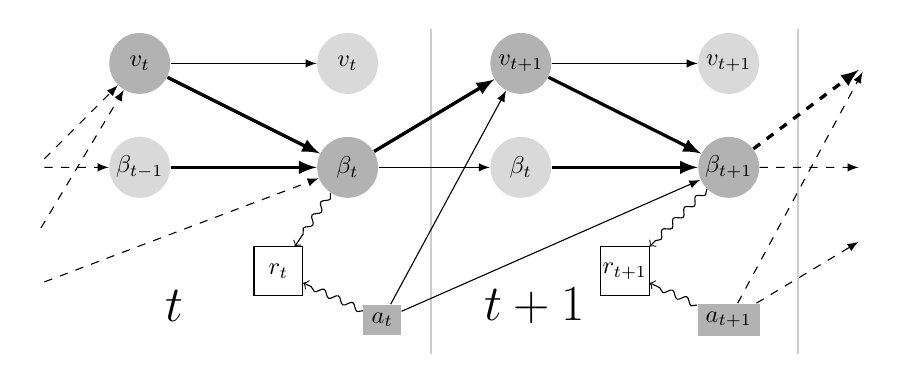
\begin{tikzpicture}[scale=0.88,transform shape]
%%%%%%%%%%%%%%%%%%%%%%%%%%%%%%%%%%%%%%%%%%%%%%%%%%%%%%%%%%%%%%
%TIME/BACKGROUND
\coordinate (middleTop) at (5.7,3);
\coordinate (middleBot) at (5.7,-1.7);
\draw[thick,color=black!20] (middleTop) -- (middleBot);
\node [font=\huge] (statet) at (2,-1) {$t$};
\coordinate (middleTop2) at (11,3);
\coordinate (middleBot2) at (11,-1.7);
\draw[thick,color=black!20] (middleTop2) -- (middleBot2);
\node [font=\huge] (statetplus1) at (7.2,-1) {$t+1$};

%%%%%%%%%%%%%%%%%%%%%%%%%%%%%%%%%%%%%%%%%%%%%%%%%%%%%%%%%%%%%%
%vertex
%vars
\tikzstyle{vertex}=[circle,fill=black!30,minimum size=25pt,inner sep=0pt]
\tikzstyle{vertex2}=[circle,fill=black!15,minimum size=25pt,inner sep=0pt]
\tikzstyle{vertex3}=[ draw, inner sep=0pt, minimum size=20pt]

%1
\node[vertex] (state1) at (1.5,2.5) {$v_t$};
\node[vertex2] (state12) at (1.5,1) {$\beta_{t-1}$};
%1bis
\node[vertex2] (state1bis) at (4.5,2.5) {$v_t$};
\node[vertex] (state12bis) at (4.5,1) {$\beta_t$};
%R1
\node[vertex3] (R1) at (3.5,-0.5) {$r_t$};

%2
\node[vertex] (state2) at (7,2.5) {$v_{t+1}$};
\node[vertex2] (state22) at (7,1) {$\beta_{t}$};

%2bis
\node[vertex2] (state2bis) at (10,2.5) {$v_{t+1}$};
\node[vertex] (state22bis) at (10,1) {$\beta_{t+1}$};
%R2
\node[vertex3] (R2) at (8.5,-0.5) {$r_{t+1}$};

%0
\node (state02) at (0,1) {};
\node (state03) at (0,2) {};
%3
\node (state3) at (12,2.5) {};
\node (state33) at (12,2) {};
\node (state32) at (12,1) {};
\node (state32bis) at (12,0) {};

%action
\node[fill=black!30] (action) at (5,-1.2) {$a_t$};
\node (action0) at (0,0) {};
\node (action02) at (0,-0.7) {};
\node[fill=black!30] (action3) at (10,-1.2) {$a_{t+1}$};

%%%%%%%%%%%%%%%%%%%%%%%%%%%%%%%%%%%%%%%%%%%%%%%%%%%%%%%%%%%%%%
%ARROWS
%1->2
\draw[->,>=latex] (state1) -- (state1bis);
\draw[->,>=latex,very thick] (state1) -- (state12bis);
\draw[->,>=latex, very thick] (state12) -- (state12bis);
%1->2bis
\draw[->,>=latex, very thick] (state12bis) -- (state2);
\draw[->,>=latex] (state12bis) -- (state22);
%0->1
\draw[->,>=latex,dashed] (state02) -- (state1);
\draw[->,>=latex,dashed] (state02) -- (state12);
%2->3
\draw[->,>=latex] (state2) -- (state2bis);
\draw[->,>=latex, very thick] (state2) -- (state22bis);
\draw[->,>=latex, very thick] (state22) -- (state22bis);
%2->3bis
\draw[->,>=latex,dashed, very thick] (state22bis) -- (state3);
\draw[->,>=latex,dashed] (state22bis) -- (state32);

%action
%1
\draw[->,>=latex] (action) -- (state2);
\draw[->,>=latex] (action) -- (state22bis);
\draw[->,decorate,decoration={snake,amplitude=.4mm,segment length=2mm,post length=1mm}] (action) -- (R1); 
%0
\draw[->,>=latex,dashed] (action0) -- (state1);
\draw[->,>=latex,dashed] (action02) -- (state12bis);
%3
\draw[->,>=latex,dashed] (action3) -- (state3);
\draw[->,>=latex,dashed] (action3) -- (state32bis);
\draw[->,decorate,decoration={snake,amplitude=.4mm,segment length=2mm,post length=1mm}] (action3) -- (R2); 

% R
\draw[->,decorate,decoration={snake,amplitude=.4mm,segment length=2mm,post length=1mm}] (state12bis) -- (R1); 
\draw[->,decorate,decoration={snake,amplitude=.4mm,segment length=2mm,post length=1mm}] (state22bis) -- (R2); 
\end{tikzpicture}
\vspace{0.3cm}
$\tilde{\mathbb{S}} =$ \\
\vspace{-0.3cm}
\textbf{beliefs}: \hspace{-0.2cm} $\beta = { \color{violet} \beta^1_v \hspace{-0.05cm} \times \hspace{-0.05cm} \ldots \hspace{-0.05cm} \times \hspace{-0.05cm} \beta^{m_v}_v } \times  { \color{gggreen} \beta^1_h \hspace{-0.05cm} \times \hspace{-0.05cm} \ldots \hspace{-0.05cm} \times \hspace{-0.05cm} \beta^{m_h}_h } \hspace{-0.07cm} \times { \color{orangee} \beta^1_f \hspace{-0.05cm} \times \hspace{-0.05cm} \ldots \hspace{-0.05cm} \times \hspace{-0.05cm} \beta^{m_f}_f } $ \\
\vspace{0.15cm}
\hspace{2cm} $\times$ \\
$ \begin{array}{c} \mbox{\textbf{visible}} \\ \mbox{\textbf{variables}} \end{array} $: $v = f \times { \color{violet} s^1_v \times \ldots \times s^{m_v}_v } \times o_1 \times \ldots \times o_{k} $.
\end{frame}

\begin{frame}
\definecolor{violet}{rgb}{0.7,0.1,0.5}
\definecolor{orangee}{rgb}{1,0.7,0.1}
\definecolor{gggreen}{rgb}{0,0.7,0.7}
\frametitle{resulting MDP in practice}
\framesubtitle{\footnotesize final structured MDP }
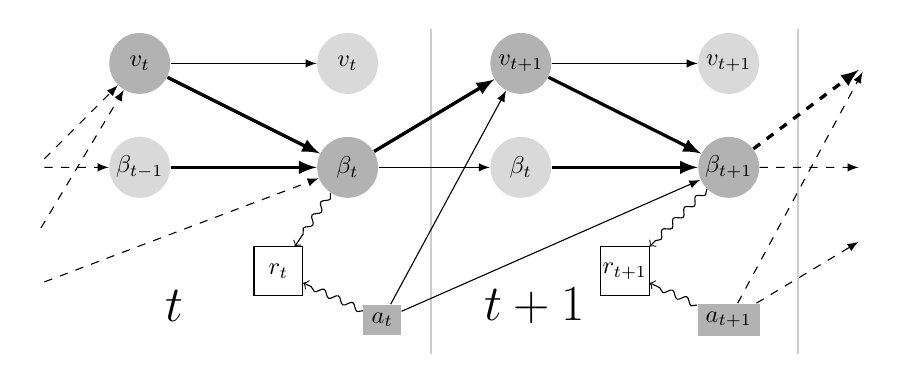
\begin{tikzpicture}[scale=0.88,transform shape]
%%%%%%%%%%%%%%%%%%%%%%%%%%%%%%%%%%%%%%%%%%%%%%%%%%%%%%%%%%%%%%
%TIME/BACKGROUND
\coordinate (middleTop) at (5.7,3);
\coordinate (middleBot) at (5.7,-1.7);
\draw[thick,color=black!20] (middleTop) -- (middleBot);
\node [font=\huge] (statet) at (2,-1) {$t$};
\coordinate (middleTop2) at (11,3);
\coordinate (middleBot2) at (11,-1.7);
\draw[thick,color=black!20] (middleTop2) -- (middleBot2);
\node [font=\huge] (statetplus1) at (7.2,-1) {$t+1$};

%%%%%%%%%%%%%%%%%%%%%%%%%%%%%%%%%%%%%%%%%%%%%%%%%%%%%%%%%%%%%%
%vertex
%vars
\tikzstyle{vertex}=[circle,fill=black!30,minimum size=25pt,inner sep=0pt]
\tikzstyle{vertex2}=[circle,fill=black!15,minimum size=25pt,inner sep=0pt]
\tikzstyle{vertex3}=[ draw, inner sep=0pt, minimum size=20pt]

%1
\node[vertex] (state1) at (1.5,2.5) {$v_t$};
\node[vertex2] (state12) at (1.5,1) {$\beta_{t-1}$};
%1bis
\node[vertex2] (state1bis) at (4.5,2.5) {$v_t$};
\node[vertex] (state12bis) at (4.5,1) {$\beta_t$};
%R1
\node[vertex3] (R1) at (3.5,-0.5) {$r_t$};

%2
\node[vertex] (state2) at (7,2.5) {$v_{t+1}$};
\node[vertex2] (state22) at (7,1) {$\beta_{t}$};

%2bis
\node[vertex2] (state2bis) at (10,2.5) {$v_{t+1}$};
\node[vertex] (state22bis) at (10,1) {$\beta_{t+1}$};
%R2
\node[vertex3] (R2) at (8.5,-0.5) {$r_{t+1}$};

%0
\node (state02) at (0,1) {};
\node (state03) at (0,2) {};
%3
\node (state3) at (12,2.5) {};
\node (state33) at (12,2) {};
\node (state32) at (12,1) {};
\node (state32bis) at (12,0) {};

%action
\node[fill=black!30] (action) at (5,-1.2) {$a_t$};
\node (action0) at (0,0) {};
\node (action02) at (0,-0.7) {};
\node[fill=black!30] (action3) at (10,-1.2) {$a_{t+1}$};

%%%%%%%%%%%%%%%%%%%%%%%%%%%%%%%%%%%%%%%%%%%%%%%%%%%%%%%%%%%%%%
%ARROWS
%1->2
\draw[->,>=latex] (state1) -- (state1bis);
\draw[->,>=latex,very thick] (state1) -- (state12bis);
\draw[->,>=latex, very thick] (state12) -- (state12bis);
%1->2bis
\draw[->,>=latex, very thick] (state12bis) -- (state2);
\draw[->,>=latex] (state12bis) -- (state22);
%0->1
\draw[->,>=latex,dashed] (state02) -- (state1);
\draw[->,>=latex,dashed] (state02) -- (state12);
%2->3
\draw[->,>=latex] (state2) -- (state2bis);
\draw[->,>=latex, very thick] (state2) -- (state22bis);
\draw[->,>=latex, very thick] (state22) -- (state22bis);
%2->3bis
\draw[->,>=latex,dashed, very thick] (state22bis) -- (state3);
\draw[->,>=latex,dashed] (state22bis) -- (state32);

%action
%1
\draw[->,>=latex] (action) -- (state2);
\draw[->,>=latex] (action) -- (state22bis);
\draw[->,decorate,decoration={snake,amplitude=.4mm,segment length=2mm,post length=1mm}] (action) -- (R1); 
%0
\draw[->,>=latex,dashed] (action0) -- (state1);
\draw[->,>=latex,dashed] (action02) -- (state12bis);
%3
\draw[->,>=latex,dashed] (action3) -- (state3);
\draw[->,>=latex,dashed] (action3) -- (state32bis);
\draw[->,decorate,decoration={snake,amplitude=.4mm,segment length=2mm,post length=1mm}] (action3) -- (R2); 

% R
\draw[->,decorate,decoration={snake,amplitude=.4mm,segment length=2mm,post length=1mm}] (state12bis) -- (R1); 
\draw[->,decorate,decoration={snake,amplitude=.4mm,segment length=2mm,post length=1mm}] (state22bis) -- (R2); 
\end{tikzpicture}
\definecolor{violet}{rgb}{0.7,0.1,0.5}
\definecolor{orangee}{rgb}{1,0.7,0.1}
\definecolor{gggreen}{rgb}{0,0.7,0.7}
%$\# \mathbb{S} \cdot \log_2 \paren{ n^{2} } \ll \log_2 \paren{ n^{\# \mathcal{S}} } $
$\#$ \textbf{factorized model}'s variables: $ \# \mathbb{O} \hspace{-0.01cm} + \hspace{-0.01cm} {\color{violet}\#\mathbb{S}_v} +$\\
$\hspace{0.5cm} \displaystyle + {\color{gggreen}\sum_{i=1}^{\# \mathbb{O}_h} \Big\lceil \log_2 \big( \lambda^{2^{p_i}} - (\lambda-1)^{2^{p_i}} \big) \Big\rceil} + {\color{orangee} \# \mathbb{S}_f \cdot \Big\lceil \log_2 \paren{ 2\lambda-1 } \Big\rceil}$ \\
\vspace{0.2cm}
\hspace{0.2cm} { \color{red} $\ll$} \hspace{0.7cm} $\#$ \textbf{initial hybrid model}'s variables: \\
\hspace{5.1cm} $\Big\lceil \log_2 \big( \lambda^{ 2^{\# \mathbb{S}} } - (\lambda-1)^{ 2^{\# \mathbb{S}} } \big) \Big\rceil$\\
\end{frame}

\begin{frame}
\definecolor{violet}{rgb}{0.7,0.1,0.5}
\definecolor{orangee}{rgb}{1,0.7,0.1}
\definecolor{gggreen}{rgb}{0,0.7,0.7}
\frametitle{resulting MDP in practice}
\framesubtitle{\footnotesize final structured MDP}
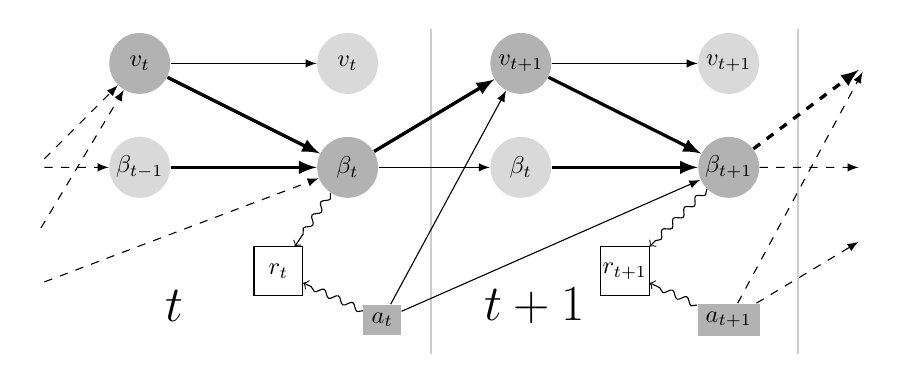
\begin{tikzpicture}[scale=0.88,transform shape]
%%%%%%%%%%%%%%%%%%%%%%%%%%%%%%%%%%%%%%%%%%%%%%%%%%%%%%%%%%%%%%
%TIME/BACKGROUND
\coordinate (middleTop) at (5.7,3);
\coordinate (middleBot) at (5.7,-1.7);
\draw[thick,color=black!20] (middleTop) -- (middleBot);
\node [font=\huge] (statet) at (2,-1) {$t$};
\coordinate (middleTop2) at (11,3);
\coordinate (middleBot2) at (11,-1.7);
\draw[thick,color=black!20] (middleTop2) -- (middleBot2);
\node [font=\huge] (statetplus1) at (7.2,-1) {$t+1$};

%%%%%%%%%%%%%%%%%%%%%%%%%%%%%%%%%%%%%%%%%%%%%%%%%%%%%%%%%%%%%%
%vertex
%vars
\tikzstyle{vertex}=[circle,fill=black!30,minimum size=25pt,inner sep=0pt]
\tikzstyle{vertex2}=[circle,fill=black!15,minimum size=25pt,inner sep=0pt]
\tikzstyle{vertex3}=[ draw, inner sep=0pt, minimum size=20pt]

%1
\node[vertex] (state1) at (1.5,2.5) {$v_t$};
\node[vertex2] (state12) at (1.5,1) {$\beta_{t-1}$};
%1bis
\node[vertex2] (state1bis) at (4.5,2.5) {$v_t$};
\node[vertex] (state12bis) at (4.5,1) {$\beta_t$};
%R1
\node[vertex3] (R1) at (3.5,-0.5) {$r_t$};

%2
\node[vertex] (state2) at (7,2.5) {$v_{t+1}$};
\node[vertex2] (state22) at (7,1) {$\beta_{t}$};

%2bis
\node[vertex2] (state2bis) at (10,2.5) {$v_{t+1}$};
\node[vertex] (state22bis) at (10,1) {$\beta_{t+1}$};
%R2
\node[vertex3] (R2) at (8.5,-0.5) {$r_{t+1}$};

%0
\node (state02) at (0,1) {};
\node (state03) at (0,2) {};
%3
\node (state3) at (12,2.5) {};
\node (state33) at (12,2) {};
\node (state32) at (12,1) {};
\node (state32bis) at (12,0) {};

%action
\node[fill=black!30] (action) at (5,-1.2) {$a_t$};
\node (action0) at (0,0) {};
\node (action02) at (0,-0.7) {};
\node[fill=black!30] (action3) at (10,-1.2) {$a_{t+1}$};

%%%%%%%%%%%%%%%%%%%%%%%%%%%%%%%%%%%%%%%%%%%%%%%%%%%%%%%%%%%%%%
%ARROWS
%1->2
\draw[->,>=latex] (state1) -- (state1bis);
\draw[->,>=latex,very thick] (state1) -- (state12bis);
\draw[->,>=latex, very thick] (state12) -- (state12bis);
%1->2bis
\draw[->,>=latex, very thick] (state12bis) -- (state2);
\draw[->,>=latex] (state12bis) -- (state22);
%0->1
\draw[->,>=latex,dashed] (state02) -- (state1);
\draw[->,>=latex,dashed] (state02) -- (state12);
%2->3
\draw[->,>=latex] (state2) -- (state2bis);
\draw[->,>=latex, very thick] (state2) -- (state22bis);
\draw[->,>=latex, very thick] (state22) -- (state22bis);
%2->3bis
\draw[->,>=latex,dashed, very thick] (state22bis) -- (state3);
\draw[->,>=latex,dashed] (state22bis) -- (state32);

%action
%1
\draw[->,>=latex] (action) -- (state2);
\draw[->,>=latex] (action) -- (state22bis);
\draw[->,decorate,decoration={snake,amplitude=.4mm,segment length=2mm,post length=1mm}] (action) -- (R1); 
%0
\draw[->,>=latex,dashed] (action0) -- (state1);
\draw[->,>=latex,dashed] (action02) -- (state12bis);
%3
\draw[->,>=latex,dashed] (action3) -- (state3);
\draw[->,>=latex,dashed] (action3) -- (state32bis);
\draw[->,decorate,decoration={snake,amplitude=.4mm,segment length=2mm,post length=1mm}] (action3) -- (R2); 

% R
\draw[->,decorate,decoration={snake,amplitude=.4mm,segment length=2mm,post length=1mm}] (state12bis) -- (R1); 
\draw[->,decorate,decoration={snake,amplitude=.4mm,segment length=2mm,post length=1mm}] (state22bis) -- (R2); 
\end{tikzpicture}
\definecolor{violet}{rgb}{0.7,0.1,0.5}
\definecolor{orangee}{rgb}{1,0.7,0.1}
\definecolor{gggreen}{rgb}{0,0.7,0.7}
%$\# \mathbb{S} \cdot \log_2 \paren{ n^{2} } \ll \log_2 \paren{ n^{\# \mathcal{S}} } $
$\#$ \textbf{factorized model}'s variables:\\
\hspace{1cm} $ \leqslant \displaystyle \# \mathbb{O} + { \color{violet} \# \mathbb{S}_v} + { \color{gggreen} \sum_{i=1}^{\# \mathbb{O}_h} \log_2 (\lambda) \cdot 2^{p_i} } + { \color{orangee} \# \mathbb{S}_f \cdot (1 + \log_2(\lambda)) } $ \\
\vspace{0.3cm}
\hspace{0.2cm} { \color{red} $\ll$} \hspace{0.7cm} $\#$ \textbf{initial hybrid model}'s variables: \\
\hspace{5.1cm} $\geqslant \log_2(\lambda) \cdot (2^{\# \mathbb{S}}-1)$.
\end{frame}

\section{Conclusion/Perspectives}
\begin{frame}
\frametitle{Conclusion}
\begin{block}{POMDP $\xrightarrow{ \mbox{\footnotesize \textbf{translation}} }$ MDP with finite state space}
\begin{itemize}
\item transition probabilities on the \textbf{possibilistic belief states};
\visible<2->{
\item \textbf{pessimistic} evaluation of the \textbf{rewards} \\
(Choquet integral);
}
\visible<3->{ 
\item factorized POMDP $\xrightarrow{ \mbox{\footnotesize \textbf{translation}} }$ \textbf{factorized} MPD.
}
\end{itemize}
\end{block}
\visible<4->{
\textbf{perspectives:} 
\begin{itemize}
\item IPPC problems (factorized POMDPs);
\visible<5->{
\item tests of this approach: 
\begin{enumerate}
\item \textbf{simplification:} $\pi$ distributions definition\\
($\pi$-normalization, pignistic transformation,\\ 
most specific, \ldots);
\item \textbf{imprecision:} robust in practice?
\end{enumerate}
}
\end{itemize}
}
\end{frame}

% questions
\frame{
  \vspace{2cm}
  {\huge Thank you!}

}
\end{document}
